 %   Template - Institute of Control Systems, Hamburg University of Technology
 %
 %   P. Göttsch, A. Popov
 %
 %   Updates: 	AP: 29.08.2007;  AP: 17.09.2007; AP: 16.06.2009
 %				PG: 28.08.2019;
 %


 %##########################################
 %     R E A D      M E     F I R S T  !
 %##########################################
 % beamer package and manual can be downloaded from  %
 % https://ctan.org/pkg/beamer
 %
 % Possible compilation processes:
 % LaTeX -> LueLAatex -> biber -> 2x luaLatex -> PDF
 % LaTeX -> pdfTeX -> PDF
 %##########################################


 %------------------------------------------
 % INFO:   Presentation Time -> 30 min 
 %------------------------------------------
 % INFO:   Discussion -> 15 - 20 min
 %------------------------------------------


 %%################ Document  settings ###################
 \def\isenglish{true} 		% Choose language for setting right language order for latex
\documentclass[compress]{beamer}

\mode<presentation>
{
  \usetheme{RT}
  \setbeamercovered{transparent}
  \usecolortheme{RT}
}

\setbeamertemplate{navigation symbols}{}
\setbeamertemplate{footline}[frame number]{}


\usepackage{ifthen}
\ifthenelse{\equal{\isenglish}{true}}{
	%%% English
	\usepackage[german, ngerman, english]{babel}
	\selectlanguage{english}
}{
	%%% German
	\usepackage[english, german, ngerman]{babel}
	\selectlanguage{german}
}

\usepackage{lmodern}
\usepackage{csquotes}
\usepackage{microtype}
\ifluatex
	\usepackage{fontspec}
\else
	\usepackage[utf8]{inputenc}
\fi

%% Allow usage of the part command to create different navigations parts 
\usepackage{xpatch}
\makeatletter
\xpatchcmd{\beamer@part}{\Hy@writebookmark{\the\c@section}{#1}{Outline\the\c@part}{1}{toc}}{}{}{}
\makeatother

\usepackage{appendixnumberbeamer}

\makeatletter
\AtBeginPart{%
  \beamer@tocsectionnumber=0\relax
  \setcounter{section}{0}
%   \frame{\partpage}%
}
\makeatother


 %%######## GRAPHICS Options
\graphicspath{{figures/}}				% Define the path to the figures

\usepackage{ifpdf}

 % Other figures (e.g., MATLAB  EPS or PDF figures)
\newcommand{\afig}[2]{\includegraphics[scale=#1]{#2}}

 % figures defined in TeX files
\newcommand{\tfig}[2]{\scalebox{#1}{\input{"#2.tex"}}}

\usepackage{multimedia}
\usepackage{tikz}

\usetikzlibrary{%
  arrows,%
  arrows.meta,
  shapes.misc,% wg. rounded rectangle
  shapes.arrows,
  shapes.misc,
  calc,
  plotmarks,
  chains,%
  matrix,%
  positioning,% wg. " of "
  scopes,%
  decorations.pathmorphing,% /pgf/decoration/random steps | erste Graphik
  decorations.markings,
  shadows%
}
\usetikzlibrary{external}
\tikzexternalize[prefix=figures/0externalize/] % activate!
\usepackage{pgfplots}
\pgfplotsset{compat=newest}

\newlength{\figw}
\setlength{\figw}{0.8\textwidth}
\newlength{\figh}
\setlength{\figh}{0.4\textwidth}

\newcommand{\tikzfig}[2]{
  \tikzsetnextfilename{#2}%
  \scalebox{#1}{
    \input{"figures/#2.tex"}}
}

 %%######## Logos only on Title page
% \titlegraphic{\vspace{0.1cm}\includegraphics[height=0.8cm]{admin/} \hfill 
\includegraphics[height=0.7cm]{Logo_ICS_4c}}

\titlegraphic{
	\vspace{1cm}
	\begin{minipage}{0.5\textwidth}
		\begin{flushleft} \large
			\ifthenelse{\equal{\isenglish}{true}}
			{
\includegraphics[height=0.8cm]{admin/Logo_TUHH_rgb_en}}
			{
\includegraphics[height=0.8cm]{admin/Logo_TUHH_rgb_de}}
		\end{flushleft}
	\end{minipage}
	\hfill
	\begin{minipage}{0.4\textwidth}
		\begin{flushright} \large
			
\includegraphics[height=0.8cm]{admin/Logo_ICS_4c} % Supervisor's Name
		\end{flushright}
	\end{minipage}\\[0.4cm]
}

 %%######## Other FUNCTIONS

 % Some color definitions
\setbeamercolor{greenhead}{fg=white,bg=green!80!black}%
\setbeamercolor{greenbody}{fg=black,bg=green!50!white}%

\setbeamercolor{redhead}{fg=white,bg=red!80!black}%
\setbeamercolor{redbody}{fg=black,bg=red!50!white}%


\usepackage{epstopdf}

\usepackage[style=ieee,backend=biber]{biblatex} %% bibliography    		% make all adjustments to language and packages here
\addbibresource{ics.bib}	% Literature file include

\title{Distributed Model Predictive Control}

\author[P. Paul]{Peter Paul \texorpdfstring{\\}{} {\small\texttt{peter.paul@tuhh.de}}}

\institute{
	Hamburg University of Technology\\ Institute of Control Systems
}

\date[\today]{Bachelorarbeit \\ \today}
 % (optional, should be abbreviation of conference name)

\subject{Control Systems}


 %%########################  BEGIN THE PRESENTATION ############################
\begin{document}
\begin{frame}
	\titlepage
\end{frame}

%%#########################  Motivation & Agenda ###############################
\part{Introduction}

\section{Motivation}
\label{sec:motivation}
\begin{frame}
    \frametitle{Motivation 1}
	\begin{itemize}
		\item \textbf{7} agents (double integrators)
		\item Potential functions
 		\item local controllers
 		\item input constraints
 		\item two ellipsoidal obstacles
 		\item Same initial and final position
 		\item Safety distance between agents
	\end{itemize}
\end{frame}	



%%#########################  Content ###########################################
\part{Content}

% \section{Agenda}
% \label{sec:agenda}

\begin{frame}<beamer>{Contents}
    \tableofcontents[part=2,hideallsubsections]
\end{frame}

\section{Nonpredictive Scenario}
\begin{frame}	\frametitle{Nonpredictive Scenario}
	\begin{itemize}
		\item \textbf{7} agents (double integrators)
		\item Potential functions
 		\item local controllers
 		\item input constraints
 		\item two ellipsoidal obstacles
 		\item Same initial and final position
 		\item Safety distance between agents
	\end{itemize}
\end{frame}	

\begin{frame}	\frametitle{Nonpredictive Scenario (by AT) - Simulink}
		\centering
		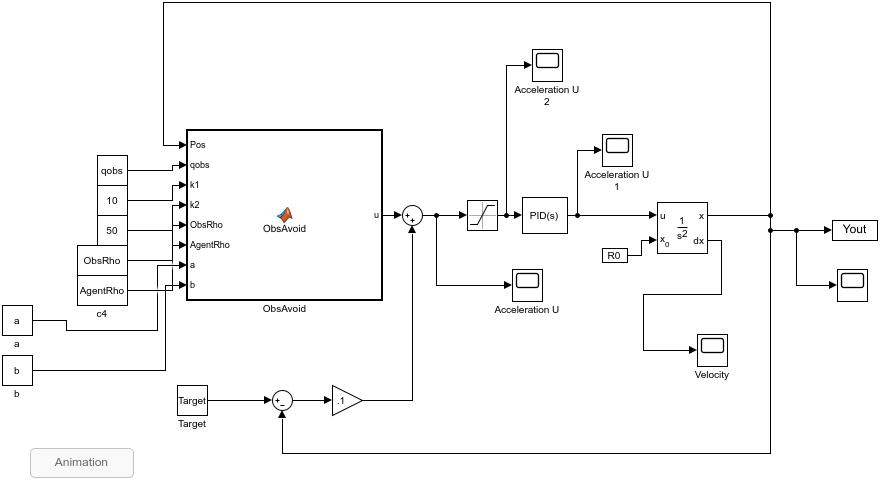
\includegraphics[scale=0.7, angle=0]{tmp30938.jpg}
\end{frame}

\section{What I want to do}

\begin{frame}	\frametitle{What I want to do}
	\begin{itemize}
		\item Continue reading and filling the table
		\item Think about how to include consensus? (Flocking, or other ideas?!) \cite{EiHoWe13d,ElAh07}
		\item if using a "global" costfunction, how to cope with iterations, are they avoidable to some extent?
	\end{itemize}
\end{frame}

\section{Conclusion and Outlook}

\subsection{Conclusion}
    \begin{frame}
        \frametitle{Conclusion}
        \begin{itemize}
            \item Continue reading and filling the table
            \item Think about how to include consensus? (Flocking, or other ideas?!)
            \item if using a "global" costfunction, how to cope with iterations, are they avoidable to some extent?
        \end{itemize}
    \end{frame}

\subsection{Outlook}
    \begin{frame}
        \frametitle{Outlook}
        \begin{itemize}
            \item Continue reading and filling the table
            \item Think about how to include consensus? (Flocking, or other ideas?!)
            \item if using a "global" costfunction, how to cope with iterations, are they avoidable to some extent?
        \end{itemize}
    \end{frame}

%%#########################  Final Slide #######################################

\begin{frame}
	\frametitle{The End}
	\centering
	Thank you very much for your attention!
\end{frame}

%%#########################  Appendix    #######################################

\appendix
\section[References]{References long Title}
\begin{frame}
	\small
	\printbibliography
\end{frame}

\section{Appendix}
\begin{frame}
    \frametitle{Appendix}
    
    \Large Here is space for further frames

\end{frame}

\end{document}